\documentclass[xcolor=dvipsnames,polish]{beamer}
%
\mode<presentation>
{
  \usetheme{CambridgeUS}

  \setbeamercovered{transparent}
}
\usefonttheme[onlylarge]{structurebold}
%\usepackage[polish]{babel}
\usepackage{polski}
\usepackage[utf8]{inputenc}
%\setbeameroption{show notes}
%
%\usepackage{times}
%\usepackage[T1]{fontenc}
%\usepackage{ae}
\usepackage{tikz}
%\usepackage{ulem}
\usepackage{color}
%\usepackage{iwona}
\usepackage{amsmath}
\usepackage{textcomp}
\usepackage{tabularx}
\usepackage{xcolor,colortbl}
\usepackage{verbatim}
\newcommand{\textapprox}{\raisebox{0.5ex}{\texttildelow}}

%
\usetikzlibrary{arrows,shapes,trees,automata,decorations.pathmorphing,matrix,backgrounds,positioning}
%
\newcommand{\marked}[1]{{\bf #1}}
\newcommand{\markerr}[1]{\textcolor{red}{#1}}


\newcommand\Wider[2][3em]{%
\makebox[\linewidth][c]{%
  \begin{minipage}{\dimexpr\textwidth+#1\relax}
  \raggedright#2
  \end{minipage}%
  }%
}

\definecolor{Gray}{gray}{0.90}
\newcolumntype{a}{>{\columncolor{Gray}}c}

%
\title[Tagery dla języka polskiego]{Tagery morfosyntaktyczne dla języka polskiego}
%
\author{Łukasz Kobyliński \and Witold Kieraś}
%
\institute[IPI PAN]{%
     Instytut Podstaw Informatyki Polskiej Akademii Nauk\\
     ul. Jana Kazimierza 5, 01-248 Warszawa, Poland}
%
\date{7.12.2015}
%
\setbeamercolor{block title}{use=structure,fg=white,bg=purple!75!black}
\setbeamercolor{block body}{use=structure,fg=black,bg=white!20!white}
%
\setbeamertemplate{section page}
{
    \begin{centering}
    \begin{beamercolorbox}[sep=12pt,center]{part title}
    \usebeamerfont{section title}\insertsection\par
    \end{beamercolorbox}
    \end{centering}
}
%
\begin{document}
\begin{frame}
  \titlepage
\end{frame}

\begin{frame}{Wprowadzenie}
\structure{Cele prezentacji}
\begin{itemize}
  \item podsumowanie obecnego stanu narzędzi do tagowania morfosyntaktycznego w języku polskim,
  \item porównanie dokładności i wykorzystywanych algorytmów z narzędziami dla innych języków europejskich,
  \item analiza jakościowa wyników działania poszczególnych tagerów,
  \item przegląd problemów, które nie zostały rozwiązane przez istniejące tagery,
  \item stwierdzenie, czy wśród dostępnych narzędzi istnieje tager o pożądanych cechach,% (następny slajd),
  \item rekomendacje dotyczące dalszych kroków.
\end{itemize}
\end{frame}

\begin{frame}{Wprowadzenie}
  \structure{Cechy pożądanego tagera (M. Woliński)}
  \vspace{0.5cm}

  Chciałbym tager, który:
   \begin{itemize}
   \item nie jest nadgorliwy, można kazać zostawić interpretacje częściowo nieujednoznacznione (np. usunąć tylko bardzo złe interpretacje),
   \item informuje o~poziomie pewności podjętych decyzji,
   \item działa na niejednoznacznej segmentacji (stworzonej przez Morfeusza lub np. będącej wynikiem zastosowania po Morfeuszu słownika wyrażeń wieloczłonowych),
   \item daje się (względnie?) łatwo zainstalować i uruchomić na wszystkich platformach, na których jest Morfeusz,
   \item da się rozszerzyć o uwzględnianie informacji o czasie powstania tekstu.
   \end{itemize}
\end{frame}

\begin{frame}
\frametitle{Plan}
\tableofcontents
\end{frame}

\section{Tagery języka polskiego -- przegląd rozwiązań}
\frame{\sectionpage}

\begin{frame}{Czym jest tagowanie -- przypomnienie}
  \structure{Segment (token)} -- wyraz lub jego fragment, znak interpunkcyjny, ciąg cyfr
lub symboli. Segmenty są ciągłe oraz rozłączne.
  \vspace{0.5cm}

  \structure{Znacznik morfosyntaktyczny (tag)} -- symbol, który można przypisać segmentowi, określający jego własności morfologiczno-składniowe.
  \vspace{0.5cm}

  \structure{Znakowanie morfosyntaktyczne (tagowanie)} -- zadanie przypisania ciągowi segmentów ciągu znaczników morfosyntaktycznych.
  \vspace{1cm}

  \structure{Segmentacja} $\Rightarrow$ \structure{Analiza morfosyntaktyczna} $\Rightarrow$ \structure{Ujednoznacznianie morfosyntaktyczne}
\end{frame}

\begin{frame}{Pełny stos przetwarzania}
  \vspace{-0.25cm}
  \begin{center}
  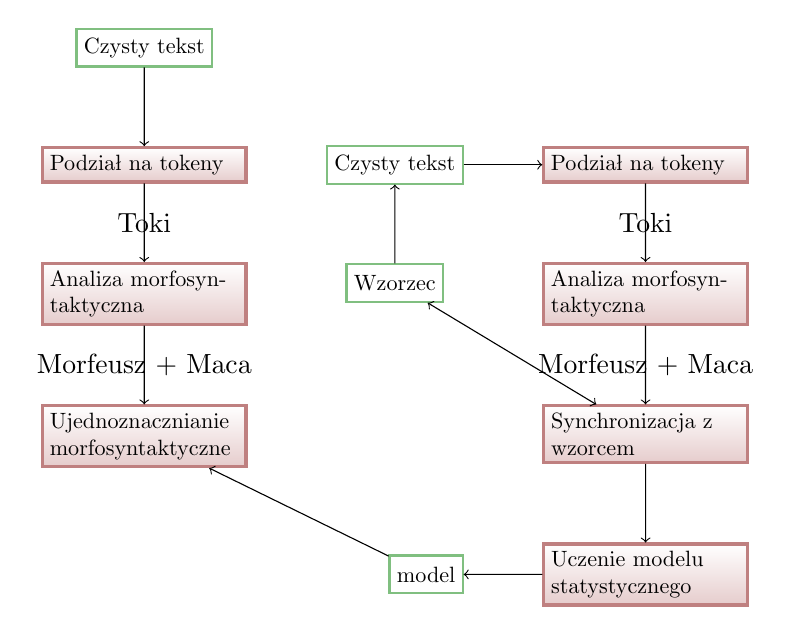
\begin{tikzpicture}[scale=0.8,
  akcja/.style={
  % The shape:
  rectangle,
  % The size:
  %minimum size=6mm,
  text width=3cm,
  % The border:
  very thick,
  draw=red!50!black!50, % 50% red and 50% black,
  % and that mixed with 50% white
  % The filling:
  top color=white, % a shading that is white at the top...
  bottom color=red!50!black!20, % and something else at the bottom
  % Font
  %font=\itshape
  scale=0.8
  },
  zasob/.style={
  % The shape:
  rectangle,
  % The size:
  minimum size=6mm,
  %text width=3cm,
  % The border:
  thick,
  draw=green!50!black!50, % 50% red and 50% black,
  % and that mixed with 50% white
  % The filling:
  top color=white, % a shading that is white at the top...
  %bottom color=red!50!black!20, % and something else at the bottom
  % Font
  %font=\itshape
  scale=0.8
  }]
  \node (T1) [akcja] {Podział na tokeny};
  \node (txtT) [zasob,above=of T1] {Czysty tekst};
  \node (T2) [akcja,below=of T1] {Analiza morfosyntaktyczna};
  \node (T3) [akcja,below=of T2] {Ujednoznacznianie\\ morfosyntaktyczne};

  \draw[->] (txtT) to (T1);
  \draw[->] (T1) to node {Toki} (T2);
  \draw[->] (T2) to node {Morfeusz + Maca} (T3);

  \node (txtL) [zasob,right=of T1] {Czysty tekst};
  \node (wzorzec) [zasob,below=of txtL] {Wzorzec};

  \node (L1) [akcja,right=of txtL] {Podział na tokeny};
  \node (L2) [akcja,below=of L1] {Analiza morfosyntaktyczna};
  \node (L3) [akcja,below=of L2] {Synchronizacja z wzorcem};
  \node (L4) [akcja,below=of L3] {Uczenie modelu statystycznego};
  \draw[->] (L1) to node {Toki} (L2);
  \draw[->] (L2) to node {Morfeusz + Maca} (L3);
  \draw[->] (L3) to (L4);

  \draw[->] (wzorzec) to (txtL);
  \draw[->] (txtL) to (L1);
  \draw[<->] (L3) to (wzorzec);

  \node (model) [zasob,left=of L4] {model};
  \draw[->] (L4) to (model);
  \draw[->] (model) to (T3);
  \end{tikzpicture}
  \end{center}
\end{frame}

\begin{frame}{Tagery morfosyyntaktyczne dla języka polskiego}
\structure{Tagery ,,archiwalne''}
\vspace{0.5cm}

Dostosowane do tagsetu IPI PAN, modele uczone na korpusie IPI.
\begin{itemize}
\item tager Ł. Dębowskiego -- statystyczny tager trigramowy,\\
$weak\ correctness = 90,59\%$
\item TaKIPI -- tager hybrydowy, oparty na drzewach decyzyjnych, częstości unigramów i ręcznie utworzonych regułach.\\
$weak\ correctness = 91.30\%$
\end{itemize}
\end{frame}

\begin{frame}{Tagery morfosyntaktyczne dla języka polskiego}
\structure{Tagery uwzględniające tagset NKJP}
\begin{itemize}
\item Pantera [Acedański 2010] -- adaptacja algorytmu Brilla do języków bogatych morfologicznie, takich jak polski,
\item WMBT [Radziszewski and Śniatowski 2011] -- tager oparty na uczeniu pamięciowym, rozbudowany o wielowarstwowość dla uwzględnienia wielu atrybutów znakowania w języku polskim,
\item Concraft [Waszczuk 2012] -- tager warstwowy, oparty na Conditional Random Fields (CRF); wyniki dezambiguacji morfosyntaktycznej przekazywane są z jednej warstwy do drugiej,
\item WCRFT [Radziszewski 2013] -- również oparty na CRF; osobne modele wykorzystywane są do dezambiguacji poszczególnych atrybutów opisu morfosyntaktycznego,
\end{itemize}
\end{frame}

\begin{frame}{Tagery morfosyntaktyczne dla języka polskiego}
\structure{Modele dla tagerów zaimplementowanych dla innych języków}
\begin{itemize}
\item TnT Tagger -- statystyczny tager trigramowy, model dla PL przygotowany przez M. Miłkowskiego,\\
dokładność ,,ok. 88\%'',\\
{\footnotesize \url{http://zil.ipipan.waw.pl/NKJP\%20model\%20for\%20TnT\%20Tagger}}
\item OpenNLP -- tager maksimum entropii, model dla PL przygotowany przez P. Pęzika (nie jest udostępniony publicznie).
{\footnotesize \url{http://clarin.pelcra.pl/tools/tagger}}
\end{itemize}
\end{frame}

\begin{frame}{Tager Brilla -- zasada działania}
\structure{Uczenie tagera}
\begin{itemize}
  \item wytrenuj tager unigramowy na podstawie zbioru uczącego,
  \item otaguj zbiór rozwojowy za pomocą tagera unigramowego,
  \item iteracyjnie znajdź transformacje, które mogą poprawić największą liczbę błędów, wprowadzając jednocześnie jak najmniej pomyłek
  \item zachowaj zbiór najlepszych transformacji -- model.
\end{itemize}
\begin{tabular}{p{8cm}|r|r}
r & good(r) & bad(r) \\ \hline
Zmień przypadek przyimka z \texttt{acc} na \texttt{loc}, jeśli kończy
się na \texttt{na} i jeden z kolejnych tokenów jest w przypadku
\texttt{loc}. & 2496 & 113 \\ \hline
Zmień przypadek przymiotnika z \texttt{loc} na \texttt{inst}, jeśli jeden z kolejnych tokenów ma przypadek \texttt{inst} i~kończy się na \texttt{em}. & 921 & 29 \\ \hline
\end{tabular}
\end{frame}

\begin{frame}{Tager Brilla -- przykładowe reguły}
\structure{Transformacje}
Zachodzą według jednego z szablonów:
\begin{itemize}
  \item $t_i := A\ if\ t_i = B \land \exists_{o \in O_1} t_{i+o} = C$
  \item $t_i := A\ if\ t_i = B \land \forall_{o \in O_2} t_{i+o} = D$
  \item $t_i := A\ if\ t_i = B$ i $i-$te słowo jest z wielkiej litery
  \item $t_i := A\ if\ t_i = B$ i $(i-1)-$te słowo jest z wielkiej litery
\end{itemize}
gdzie:
\begin{itemize}
  \item $O_1 \in \{\{1\}, \{-1\}, \{2\}, \{-2\}, \{1, 2\}, \{-1, -2\}, \{1, 2, 3\}$,\\
  $\{-1, -2, -3\}\}$,
  \item $O_2 \in \{\{-2, -1\}, \{-1, 1\}, \{1, 2\}\}$,
  \item $A, B, C, D$ -- tagi.
\end{itemize}
\end{frame}

\begin{frame}{Conditional Random Fields a inne modele grafowe}
  \begin{center}
    \includegraphics[width=0.8\textwidth]{img/pgms.png}
  \end{center}
\end{frame}

\begin{frame}{WCRFT i Concraft -- zasada działania}
\begin{columns}[t]
  \column{0.5\textwidth}
  \structure{WCRFT}
  \begin{itemize}
    \item wieloprzebiegowe ujednoznacznianie niezależnych warstw: klasa gramatyczna, liczba, przypadek, itp.
    \item modele pierwszego rzędu -- kontekst analizowany na poziomie obserwacji,
    \item cechy: forma ortograficzna (\emph{orth}), bigramy \emph{orth}, klasa gramatyczna, bigramy, trigramy \emph{orth}, przypadek, rodzaj, liczba, zgodnosć gramatyczna
  \end{itemize}
  \column{0.5\textwidth}
  \structure{Concraft}
  \begin{itemize}
    \item wprowadzenie ograniczeń co do możliwości występowania tagów w danym kontekście w algorytm CRF (ograniczony liniowy model CRF),
    \item ujednoznacznianie w dwóch warstwach wpływających na siebie (część mowy + przypadek + osoba, pozostałe kategorie gramatyczne),
    \item cechy: forma ortograficzna, dla OOV: prefiks, sufiks, pocz. zdania,
  \end{itemize}
\end{columns}
\end{frame}

\begin{frame}{Przenośność i łatwość wykorzystania}
  \begin{itemize}
    \item \structure{Concraft} instalowany i uruchamiany z wykorzystaniem Haskell Platform, która dostępna jest pod wszystkie główne systemy operacyjne,
    \item \structure{WCRFT, Pantera} -- wymagają kompilacji, proces kompilacji dostosowany do środowiska Linuksowego,
    \item \structure{WMBT} -- Python.
  \end{itemize}
  \vspace{1cm}

  \structure{Concraft, WCRFT, WMBT} -- silnie zależą od stosu Corpus2 / Toki / Maca, których kompilacja pod Windows jest możliwa, ale nietrywialna (Visual Studio).
\end{frame}

%\section{Tagery morfosyntaktyczne dla innych języków europejskich}
%\frame{\sectionpage}

\section{Tagery języka polskiego -- analiza ilościowa}
\frame{\sectionpage}

\begin{frame}{Metoda ewaluacji}
\structure{Miara jakości znakowania}
\begin{itemize}
\item ze względu na możliwość wystąpienia różnic w segmentacji pomiędzy wynikiem znakowania, a złotym standardem, wykorzystujemy dolne ograniczenie trafności (\emph{accuracy lower bound}, $Acc_{lower}$) do oceny dokładności tagerów,
\item miara ta karze wszelkie zmiany segmentacyjne w stosunku do złotego standardu i traktuje takie tokeny jako sklasyfikowane błędnie,
\item token traktowany jest jako oznakowany prawidłowo, jeśli zbiór jego interpretacji ma niepuste przecięcie ze zbiorem interpretacji zwracanych przez tager,
\item niezależne sprawdzamy dokładność dla znanych ($Acc^K_{lower}$) i nieznanych słów ($Acc^U_{lower}$), aby ocenić skuteczność ew. modułów odgadywania.
\end{itemize}
\end{frame}

\begin{frame}{Ewaluacja tagerów}
\structure{Eksperymenty na milionowym podkorpusie Narodowego Korpusu Języka Polskiego, ver. 1.1, 10-krotna walidacja krzyżowa.}
\begin{center}
\begin{tabular}{lcccc} \hline
n & Tager 		& $Acc_{lower}$	& $Acc^K_{lower}$	& $Acc^U_{lower}$	\\ \hline
1 & Pantera   & 88.95\%   & 91.22\% & 15.19\% \\
2 & WMBT	 	& 90.33\%		& 91.26\%	& 60.25\%	\\
3 & WCRFT	 	& 90.76\%		& 91.92\%	& 53.18\%	\\
4 & Concraft	& 91.07\%		& 92.06\%	& 58.81\%	\\
\end{tabular}
\end{center}
\begin{itemize}
\item $Acc_{lower}$ -- łączna dokładność,
\item $Acc^K_{lower}$ -- dokładność dla znanych słów,
\item $Acc^U_{lower}$ -- dokładność dla słów nieznanych (2,8\% Morfeusz1, 1,6\% Morfeusz2).
\end{itemize}
\end{frame}

\begin{frame}{Tagery języków europejskich -- porównanie}
  \begin{center}
  \begin{tabular}{l|l|r|r|r}
    Tager       & Język     & Rozmiar & Korpus  & Dokładność \\
                &           & tagsetu & treningowy & \\ \hline
    Concraft    & polski    & 4 000 / 1 000 & 1M    & 91,07\% \\
    Obeliks     & słoweński & 1 903 & 500k  & 91,34\% \\
    Morče       & czeski    & 3 922 / 1 571 & 2M    & 95,67\% \\
    Featurama   & czeski    & 3 922 / 1 571 & 2M    & 95,66\% \\
    Morphodita  & czeski    & 3 922 / 1 571 & 2M    & 95,75\% \\
    BI-LSTM-CRF & angielski & 36+12   & 1M   & 97,55\% \\
  \end{tabular}
  \end{center}
\end{frame}

\begin{frame}{Analiza rezultatu działania tagerów}
\structure{Porównanie wyników}
\begin{itemize}
\item Wszystkie zwracają prawidłowy tag: \marked{82,78\%} \\
{\footnotesize \underline{unikam} fin:sg:pri:imperf\\
fin:sg:pri:imperf+ fin:sg:pri:imperf+ fin:sg:pri:imperf+ fin:sg:pri:imperf+}
\item Większość zwraca prawidłowy tag: \marked{7,95\%} \\
{\footnotesize \underline{kapitalistów} subst:pl:gen:m1 \\
subst:pl:gen:m1+ subst:pl:gen:m1+ subst:pl:gen:m1+ subst:pl:acc:m1-}
\item Równowaga w głosowaniu: \marked{2,71\%} \\
{\footnotesize \underline{powolny} adj:sg:nom:m3:pos \\
adj:sg:nom:m3:pos+ adj:sg:nom:m3:pos+ adj:sg:acc:m3:pos- adj:sg:acc:m3:pos-}
\item Prawidłowy tag w mniejszości: \marked{2,38\%} \\
{\footnotesize \underline{twarzy} subst:sg:loc:f subst:sg:gen:f- subst:sg:gen:f- subst:sg:gen:f- subst:sg:loc:f+}
\item Wszystkie się mylą: \marked{4.18\%} \\
{\footnotesize \underline{biurka} subst:pl:nom:n subst:pl:acc:n- subst:pl:acc:n- subst:sg:gen:n- subst:pl:acc:n- \\
(Peggy) \underline{McCreary} subst:sg:nom:f \\
subst:sg:gen:f- subst:sg:gen:n- subst:sg:nom:n- subst:sg:acc:m1-}
\end{itemize}
\end{frame}

\begin{frame}{Podział na klasy gramatyczne}
\begin{center}
\begin{tabular}{llllll}
 &  & \multicolumn{4}{c}{$Acc_{lower}$ (\%)} \\
klasa & liczność & PANTERA & WMBT & WCRFT & Concraft \\
\hline
subst & 331570 & 85,21 & 86,25 & 87,36 & 88,29 \\
interp & 223542 & 99,63 & 99,97 & 99,97 & 99,97 \\
adj & 128703 & 76,53 & 81,10 & 81,56 & 82,52 \\
prep & 115818 & 97,04 & 97,28 & 97,54 & 98,05 \\
qub & 68079 & 92,98 & 93,82 & 92,91 & 92,92 \\
fin & 59458 & 98,64 & 98,70 & 98,81 & 98,94 \\
praet & 53326 & 90,90 & 88,96 & 89,80 & 89,69 \\
conj & 44840 & 95,17 & 95,41 & 94,61 & 93,96 \\
adv & 42750 & 95,31 & 95,59 & 95,29 & 94,77 \\
inf & 19213 & 98,91 & 99,20 & 99,09 & 99,14 \\
comp & 17842 & 97,26 & 97,29 & 96,84 & 96,88 \\
num & 16160 & 33,40 & 56,40 & 60,32 & 55,99 \\
\end{tabular}
\end{center}
\end{frame}

\begin{frame}{Podział na klasy gramatyczne}
  \structure{Concraft: błąd wyboru klasy vs błąd w ramach klasy (test: 100k)}
  \begin{center}
    \includegraphics[width=\textwidth]{img/ctag_errs.png}
  \end{center}
\end{frame}

\begin{frame}{Najczęstsze błędy}
  \structure{Concraft: najczęstsze błędy wyboru klasy gramatycznej}
  \begin{center}
  \begin{tabular}{llrr}
    Concraft & NKJP & liczność & \% błędów \\ \hline
    adj & subst & 199 & 1.9422 \\
    conj & qub & 178 & 1.7373 \\
    subst & adj & 162 & 1.5811 \\
    adv & qub & 159 & 1.5518 \\
    subst & ger & 152 & 1.4835 \\
    qub & conj & 151 & 1.4737 \\
    subst & brev & 140 & 1.3664 \\
    ger & subst & 128 & 1.2493 \\
    num & adj & 108 & 1.0541 \\
    ppas & adj & 108 & 1.0541 \\
    qub & adv & 91 & 0.8882 \\
    adj & ppas & 71 & 0.6930 \\
    adj & num & 71 & 0.6930 \\
  \end{tabular}
\end{center}
\end{frame}

\begin{frame}{Najczęstsze błędy}
  \structure{Concraft: najczęstsze błędy doboru tagu w ramach klasy \texttt{subst}}
  \begin{center}
  \begin{tabular}{llrr}
    Concraft & NKJP & liczność & \% błędów \\ \hline
    sg:nom:m3 & sg:acc:m3 & 191 & 1.8641 \\
    sg:acc:m3 & sg:nom:m3 & 153 & 1.4933 \\
    sg:acc:n & sg:nom:n & 134 & 1.3078 \\
    sg:nom:n & sg:acc:n & 117 & 1.1419 \\
    pl:nom:m3 & pl:acc:m3 & 89 & 0.8686 \\
    pl:acc:f & pl:nom:f & 78 & 0.7613 \\
    pl:nom:f & pl:acc:f & 71 & 0.6930 \\
    pl:acc:m3 & pl:nom:m3 & 68 & 0.6637 \\
    sg:gen:m1 & sg:acc:m1 & 67 & 0.6539 \\
    sg:acc:m1 & sg:gen:m1 & 53 & 0.5173 \\
    pl:nom:n & pl:acc:n & 48 & 0.4685 \\
    sg:gen:f & pl:gen:f & 47 & 0.4587 \\
  \end{tabular}
  \end{center}
\end{frame}

\begin{frame}{Najczęstsze błędy}
  \structure{Concraft: najczęstsze błędy doboru tagu w ramach klasy \texttt{adj}}
  \begin{center}
  \begin{tabular}{llrr}
    Concraft & NKJP & liczność & \% błędów \\ \hline
    sg:nom:m3:pos & sg:acc:m3:pos & 90 & 0.8784 \\
    sg:acc:m3:pos & sg:nom:m3:pos & 72 & 0.7027 \\
    sg:nom:m1:pos & sg:nom:m3:pos & 57 & 0.5563 \\
    sg:nom:n:pos & sg:acc:n:pos & 51 & 0.4978 \\
    pl:nom:m3:pos & pl:acc:m3:pos & 49 & 0.4782 \\
    pl:nom:f:pos & pl:acc:f:pos & 46 & 0.4490 \\
    pl:acc:f:pos & pl:nom:f:pos & 44 & 0.4294 \\
    sg:nom:m3:pos & sg:nom:m1:pos & 42 & 0.4099 \\
    sg:acc:n:pos & sg:nom:n:pos & 32 & 0.3123 \\
    pl:acc:m3:pos & pl:nom:m3:pos & 28 & 0.2733 \\
    pl:nom:n:pos & pl:acc:n:pos & 27 & 0.2635 \\
    pl:nom:m3:pos & pl:nom:f:pos & 25 & 0.2440 \\
    pl:acc:n:pos & pl:nom:n:pos & 21 & 0.2050 \\
  \end{tabular}
  \end{center}
\end{frame}

\begin{frame}{Rozmiar danych treningowych}
  \structure{TnT Tagger} -- NEGRA corpus, 30 000 tokenów testowych.
  \begin{center}
    \includegraphics[width=\textwidth]{img/tnt_lcurve.png}
  \end{center}
\end{frame}

\begin{frame}{Rozmiar danych treningowych}
  \structure{MBT Tagger} -- WSJ corpus, kroswalidacja krzyżowa
  \begin{center}
    \includegraphics[width=0.8\textwidth]{img/mbt_lcurve.png}
  \end{center}
\end{frame}

\begin{frame}{Rozmiar danych treningowych}
  \structure{Concraft} -- NKJP 1M, 100 000 tokenów testowych.
  \begin{center}
    \includegraphics[width=0.8\textwidth]{img/concraft_lcurve.png}
  \end{center}
\end{frame}

\begin{frame}{Problem niejednoznaczności segmentacji}
  \structure{Na czym polega problem?}\\
  \includegraphics[width=\textwidth]{img/segm_amb1.png}
\end{frame}

\begin{frame}{Problem niejednoznaczności segmentacji}
  \structure{Jak często występują niejednoznaczności?}\\
  Korpus NKJP 1M, Morfeusz 1 SGJP:\\
  645 wystąpień na 1 099 915 segmentów (0.0586\%)
  \begin{columns}[c]
    \column{.3\textwidth}
    \begin{center}
      \footnotesize
      \begin{tabular}{l|r}
      kiedyś & 234 / \markerr{1} \\
      gdzieś & 172 / \markerr{1} \\
      miałem & 99 / \markerr{98} \\
      udziałem & 40 / 0 \\
      musiałem & 28 / \markerr{28} \\
      sms-a & 6 / 0 \\
      działam & 6 / 0\\
      doń & 5 / \markerr{4} \\
      tyłem & 4 / 0 \\
      pis-em & 4 / 0 \\
      podziałem & 3 / 0 \\
      piekłem & 3 / 0 \\
      czekałem & 3 / \markerr{3} \\
      jadłem & 3 / \markerr{3} \\
      \end{tabular}
    \end{center}
    \column{.3\textwidth}
    \begin{center}
      \footnotesize
      \begin{tabular}{l|r}
        pis-owi & 3 \\
        winnym & 2 \\
        prl-em & 2 \\
        wyłom & 2 \\
        rozdziałem & 2 \\
        hiv-em & 2 \\
        pit-ów & 2 \\
        działem & 1 \\
        rop-em & 1 \\
        tir-a & 1 \\
        kor-owcy & 1 \\
        urm-em & 1 \\
        kor-em & 1 \\
        dj-a & 1 \\
      \end{tabular}
    \end{center}
    \column{.3\textwidth}
    \begin{center}
      \footnotesize
      \begin{tabular}{l|r}
        ipn-em & 1 \\
        sms-ów & 1 \\
        pgr-ach & 1 \\
        zus-em & 1 \\
        vat-em & 1 \\
        siadłem & 1 \\
        msz-ów & 1 \\
        zoz-ów & 1 \\
        mosir-em & 1 \\
        vip-om & 1 \\
        msz-ecie & 1 \\
        zoz-owi & 1 \\
        czemuś & 1 \\
      \end{tabular}
    \end{center}
  \end{columns}
\end{frame}

\begin{frame}{Problem niejednoznaczności segmentacji}
  \structure{Jak często występują niejednoznaczności?}\\
  Próbka 100M NKJP, Morfeusz 1 SGJP:\\
  40 354 wystąpień na 101 052 527 segmentów (0.0399\%)
  \begin{columns}[c]
    \column{.3\textwidth}
    \begin{center}
      \footnotesize
      \begin{tabular}{l|r}
        kiedyś & 12751 \\
        miałem & 8350 \\
        gdzieś & 6171 \\
        udziałem & 4988 \\
        musiałem & 2173 \\
        czekałem & 537 \\
        tyłem & 523 \\
        doń & 414 \\
        podziałem & 411 \\
        sms-a & 357 \\
        vip-ów & 305 \\
        winnym & 256 \\
        sms-ów & 207 \\
        jadłem & 199 \\
      \end{tabular}
    \end{center}
    \column{.3\textwidth}
    \begin{center}
      \footnotesize
      \begin{tabular}{l|r}
        czemuś & 171 \\
        działam & 153 \\
        działem & 151 \\
        piekłem & 130 \\
        zus-em & 95 \\
        sms-em & 95 \\
        tir-ów & 93 \\
        zoz-ów & 86 \\
        tir-a & 85 \\
        zus-owi & 82 \\
        azs-em & 81 \\
        vat-em & 76 \\
        rozdziałem & 76 \\
        wyłom & 65 \\
      \end{tabular}
    \end{center}
    \column{.3\textwidth}
    \begin{center}
      \footnotesize
      \begin{tabular}{l|r}
        pit-ów & 65 \\
        Łks-em & 60 \\
        pis-em & 44 \\
        siadłem & 43 \\
        skok-i & 39 \\
        gks-em & 39 \\
        padłem & 36 \\
        pgr-ów & 30 \\
        vip-a & 30 \\
        pis-owi & 28 \\
        skok-ów & 24 \\
        pks-em & 24 \\
        dj-ów & 20 \\
        dj-e & 20 \\
      \end{tabular}
    \end{center}
  \end{columns}
\end{frame}

\begin{frame}{Problem niejednoznaczności segmentacji}
  \structure{Jak często występują niejednoznaczności?}\\
  Korpus NKJP 1M, Morfeusz 2:\\
  2583 wystąpień na 1 099 282 segmentów (0.2350\%)
  \begin{columns}[c]
    \column{.3\textwidth}
    \begin{center}
      \footnotesize
      \begin{tabular}{l|r}
        coś & 777 \\
        ktoś & 382 \\
        czym & 334 \\
        kiedyś & 234 \\
        gdzieś & 172 \\
        miałem & 99 \\
        czegoś & 97 \\
        kogoś & 82 \\
        czymś & 63 \\
        kimś & 42 \\
%        gdybym & 40 \\
        udziałem & 40 \\
        %żebym & 39 \\
        %żebyś & 34 \\
      \end{tabular}
    \end{center}
    \column{.3\textwidth}
    \begin{center}
      \footnotesize
      \begin{tabular}{l|r}
        komuś & 31 \\
%        gdybyśmy & 19 \\
        tom & 19 \\
        %żebyśmy & 12 \\
 %       gdybyś & 7 \\
        działam & 6 \\
        jam & 5 \\
        doń & 5 \\
        oścież & 5 \\
 %       gdybyście & 4 \\
        tyłem & 4 \\
        musiałem & 3 \\
        podziałem & 3 \\
        piekłem & 3 \\
       czekałem & 3 \\
      \end{tabular}
    \end{center}
    \column{.3\textwidth}
    \begin{center}
      \footnotesize
      \begin{tabular}{l|r}

        jadłem & 3 \\
        rozdziałem & 2 \\
        wyłom & 2 \\
        bom & 2 \\
        %żebyście & 2 \\
        coście & 1 \\
        czyżbyś & 1 \\
        czyżem & 1 \\
        siadłem & 1 \\
        czemuś & 1 \\
        działem & 1 \\
      \end{tabular}
    \end{center}
  \end{columns}
\end{frame}

\begin{frame}{Problem niejednoznaczności segmentacji}
  \structure{Możliwe rozwiązania: tagset pośredni (A. Radziszewski).}
  Wprowadźmy tagset pośredni, który pozwoli uniknąć części niejednoznaczności
  \begin{center}
  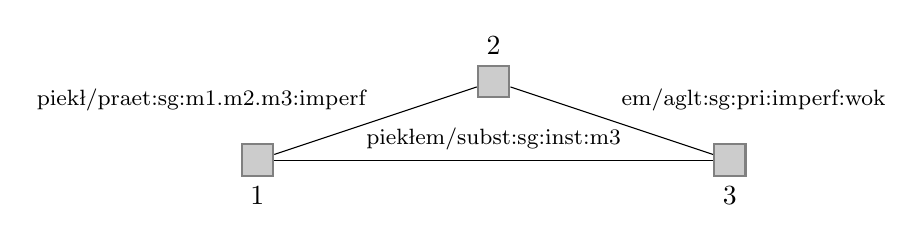
\begin{tikzpicture}[auto,xscale=3,place/.style={circle,draw=blue!50,fill=blue!20,thick,
inner sep=0pt,minimum size=6mm},
transition/.style={rectangle,draw=black!50,fill=black!20,thick,
inner sep=0pt,minimum size=4mm}]
    \node[transition,label=2] (interm) at (1,1) {};
    \node[transition,label=below:1] (beg) at (0,0) {};
    \node[transition,label=below:3] (end) at (2,0) {};
    \draw (beg) to node {\footnotesize piekłem/subst:sg:inst:m3} (end);
    \draw (beg) to node {\footnotesize piekł/praet:sg:m1.m2.m3:imperf} (interm);
    \draw (interm) to node {\footnotesize em/aglt:sg:pri:imperf:wok} (end);
    \end{tikzpicture}
  \end{center}

  piekłem\\
  \hspace{1cm}piec    fin:sg:m1:pri:imperf:prt\\
  \hspace{1cm}piec    fin:sg:m2:pri:imperf:prt\\
  \hspace{1cm}piec    fin:sg:m3:pri:imperf:prt\\
  \hspace{1cm}piekło  subst:sg:inst:n\\
\end{frame}

\begin{frame}{Problem niejednoznaczności segmentacji}
  \structure{Możliwe rozwiązania: tagset pośredni}\\
  Rozwiązanie analogiczne do trybu \texttt{-p composite} w Morfeuszu 2:
  \vspace{0.5cm}

  \$ echo piekłem | morfeusz\_analyzer\\
  {[}0,1,piekł,piec:v,praet:sg:m1.m2.m3:imperf,\_,\_{]}\\
  {[}0,2,piekłem,piekło,subst:sg:inst:n2,pospolita,\_{]}\\
  {[}1,2,em,być,aglt:sg:pri:imperf:wok,\_,\_{]}\\
  \vspace{0.5cm}

  \$ echo piekłem | morfeusz\_analyzer $-$p composite\\
  {[}0,1,piekłem,piec:v,praet:sg:m1.m2.m3:pri:imperf,\_,\_
  0,1,piekłem,piekło,subst:sg:inst:n2,pospolita,\_{]}
\end{frame}

\begin{frame}{Problem niejednoznaczności segmentacji}
  \structure{Możliwe rozwiązania: dostosowanie tagera do przetwarzania DAGów}
  \vspace{0.5cm}

  Na przykład, dla tagera Concraft: konieczna jest modyfikacja całego stosu przetwarzania:
  \begin{itemize}
    \item modyfikacja istniejących formatów zapisu korpusów (XML, Plain),
    \item modyfikacja narzędzi: Corpus2, Maca,
    \item reimplementacja algorytmu w tagerze, aby był w stanie przetwarzać dane w reprezentacji grafowej.
  \end{itemize}
\end{frame}

\begin{frame}{Poziom pewności ujednoznaczniania morfosyntaktycznego}
  \structure{Oczekujemy, że: tager informuje o~poziomie pewności podjętych decyzji}\\
  Tagery oparte na metodach uczenia maszynowego mogą zwracać prawdopodobieństwa brzegowe wyboru poszczególnych interpretacji.
  \vspace{0.25cm}

  Implementacja w Concraft:\\
  \texttt{\$ \textapprox/.cabal/bin/concraft-pl\ tag\ -m\ model.gz\ <\ test.plain}

\begin{columns}[t]
    \column{0.5\textwidth}
  \scriptsize
  rzucała space\\
  \hspace{1cm}rzucać  praet:sg:f:imperf 1.000\\
  światło space\\
  \hspace{1cm}światło adv:pos 0.000\\
  \hspace{1cm}światło subst:sg:acc:n  0.929\\
  \hspace{1cm}światło subst:sg:nom:n  0.071\\
  \hspace{1cm}światło subst:sg:voc:n  0.000\\
  \column{0.5\textwidth}
  \scriptsize
  tylko space\\
  \hspace{1cm}Tylka   subst:sg:voc:f  0.000\\
  \hspace{1cm}tylko   conj    0.209\\
  \hspace{1cm}tylko   qub     0.791\\
  na    space\\
  \hspace{1cm}na      interj  0.000\\
  \hspace{1cm}na      prep:acc        1.000\\
  \hspace{1cm}na      prep:loc        0.000\\
  podłogę space\\
  \hspace{1cm}podłoga subst:sg:acc:f  1.000\\
\end{columns}

\end{frame}

\section{Tagery języka polskiego -- analiza jakościowa}
\frame{\sectionpage}

%\begin{frame}{TODO}
%\end{frame}

\begin{frame}
  \frametitle{Tagowanie w~NKJP}
W~NKJP300 zapytanie:
\begin{itemize}\small

\item<2-> \texttt{[pos=prep \& base!=temu][case=voc]}:
  5879 wyników.

\medskip

\item<3-> \texttt{[pos=prep][pos="praet|fin|inf|impt"]}: 88
271 wyników.

\medskip

\item<4-> \texttt{[pos=prep \& base!=temu \& case=\$1][pos=adj \&
    base!=który \& case!=\$1][pos=subst \& case=\$1]}: 798 794 wyników.

\medskip

\item<5-> \texttt{[pos=prep \& base!=temu \& case=\$1][pos=subst \&
    case!=\$1]}: 5 770 963 wyników.
\end{itemize}
\end{frame}

\begin{frame}
  \frametitle{Podstawa analizy}

Tagery Pantera, Concraft, WCRF i~WMBT (w~dwu wersjach)  trenowane na 90\% NKJP1M. \\

\medskip

Analiza została przeprowadzona na pozostałych 10\%  NKJP1M (ok. 120
tys. segmentów) oznakowanych
czterema tagerami w~zestawieniu z~ręcznym znakowaniem wzorcowym.

%\medskip

% Ponadto oznakowaliśmy również:
% \begin{itemize}
% \item jedną książkę reportażową z~2015 r. w~całości,
% \item próbkę tekstów ekonomicznych.
% \end{itemize}

\end{frame}

\begin{frame}[fragile]{Różne tagsety dla języka polskiego?}
  \structure{Obecnie funkcjonują równolegle dwa tagsety języka polskiego}
  \begin{itemize}
    \item tagset NKJP, używany do anotacji korpusu, a także w większości innych zasobów językowych,
    \item tagset Morfeusza.
  \end{itemize}
  \vspace{0.5cm}

  Skutkuje to sytuacją, w której w sposób niejawny dokonywana jest ciągła konwersja pomiędzy tagsetami:
  \begin{columns}[c]
    \column{0.3\textwidth}
      \footnotesize
      \begin{verbatim}
        tagset_from=sgjp
        tagset_to=nkjp
        override=n1:n
        override=n2:n
        override=n3:n
        override=p1:m1
        override=p2:n
        override=p3:n
      \end{verbatim}
    \column{0.7\textwidth}
      \footnotesize
      \begin{verbatim}
        tagset_from=morfeusz2; tagset_to=nkjp
        override=dig:num; override=nie:conj
        override=romandig:num
        override=prefa:ign
        override=prefppas:ign
        override=prefs:ign; override=prefv:ign
        override=naj:ign; override=cond:ign
        override=substa:ign
      \end{verbatim}
    \end{columns}
\end{frame}

\begin{frame}
  \frametitle{Dwa tagsety, dwa opisy}
\end{frame}


\begin{frame}
  \frametitle{Różnice słownikowe}

\begin{itemize}
\item Brak interpretacji \texttt{adv} dla: \textsc{jeszcze}, \textsc{znów},
\textsc{znowu}, \textsc{już}, \textsc{wreszcie}.

\medskip

\item Brak interpretacji \texttt{conj} dla: \textsc{dość}, \textsc{jeszcze}, \textsc{również}, \textsc{także}, \textsc{też}.

\medskip

\item Brak interpretacji \texttt{qub} dla: \textsc{absolutnie}, \textsc{generalnie}, \textsc{głównie},
\textsc{jak}, \textsc{jakoś}, \textsc{praktycznie}, \textsc{prawdopodobnie}, \textsc{przypuszczalnie},
\textsc{rzeczywiście}, \textsc{rzekomo}, \textsc{szczególnie}, \textsc{właściwie}, \textsc{wyłącznie}.

\medskip

\item Brak interpretacji \texttt{prep} dla: \textsc{blisko},
\textsc{bliżej}, \textsc{najbliżej}, \textsc{wyjąwszy},
\textsc{apropos}, \textsc{celem}, \textsc{x}…
\end{itemize}
\end{frame}

\begin{frame}
  \frametitle{Inne różnice}

  \begin{itemize}
  \item Formy
    \emph{bliska} i~\emph{swojemu} w~wyrażeniach \emph{z~bliska}
    i~\emph{po swojemu} w~NKJP są \texttt{adjp}, w~Morfeuszu zaś --- \texttt{adj}.
  \item \textsc{Półtora} w~NKJP to wyłącznie \texttt{subst},
    w~Morfeuszu --- wyłącznie \texttt{num}.
  \item Liczebniki \textsc{pół} i~\textsc{ćwierć} w~NKJP wymają liczby
    mnogiej, w~Morfeuszu 2.0 --- pojedynczej.
  \item \texttt{Burk} w~NKJP nie odpowiadają tym w~Morfeuszu,
    np. \emph{łupnia}, \emph{zamian}, \emph{przemian}, \emph{ciemku},
    \emph{jaw} są tylko formami rzeczowników. Z~drugiej strony
    \emph{Burkina} i~\emph{Faso} w~NKJP to rzeczowniki, w~Morfeuszu
    --- burkinostki, \emph{propos} w~NKJP to kublik lub przyimek,
    w~Morfeuszu --- burkinostka, itd.
  \end{itemize}


\end{frame}

\begin{frame}
  \frametitle{Najczęściej mylone znaczniki}
\begin{itemize}\small
\item\alert<2>{\texttt{subst:sg:acc:m3} vs. \texttt{subst:sg:nom:m3}}
\item \texttt{conj} vs. \texttt{qub}
\item \alert<2>{\texttt{subst:sg:acc:n} vs. \texttt{subst:sg:nom:n}}
\item \alert<4>{\texttt{adj:sg:acc:m3:pos} vs. \texttt{adj:sg:nom:m3:pos}}
\item \alert<2>{\texttt{subst:pl:acc:m3} vs. \texttt{subst:pl:nom:m3}}
\item \alert<2>{\texttt{subst:pl:acc:f} vs. \texttt{subst:pl:nom:f}}
\item \texttt{adv} vs. \texttt{qub}
\item \alert<3>{\texttt{praet:sg:m1:perf} vs. \texttt{praet:sg:m3:perf}}
\item \alert<3>{\texttt{praet:sg:m1:imperf} vs. \texttt{praet:sg:m3:imperf}}
\item \alert<2>{\texttt{subst:sg:acc:m1} vs. \texttt{subst:sg:gen:m1}}
\item \alert<2>{\texttt{subst:pl:nom:f} vs. \texttt{subst:sg:gen:f}}
\item \alert<4>{\texttt{adj:sg:nom:m1:pos} vs. \texttt{adj:sg:nom:m3:pos}}
\item  \texttt{prep:acc} vs. \texttt{prep:loc}

\end{itemize}
\end{frame}


\begin{frame}
  \frametitle{Homonimia}\scriptsize

\Wider[-1em]{
    \setlength{\tabcolsep}{2pt}
    \begin{tabular}{rl}
\rowcolor{Gray}      przekładała & \alert<2->{\textbf{paczki}} \texttt{[paczek:subst:pl:acc:m3]}
       z ręki do ręki\\ %przest. gwar.
      W~Krakowie, w~& \textbf{krypcie}
      \texttt{[krypeć:subst:pl:acc:m3]} pod kościołem księży
      pijarów\\ %brak kwal.
\rowcolor{Gray}      pokrywa śnieżna sięga pół & \textbf{metra}
      \texttt{[metro:subst:sg:gen:n]} . \\ % brak kwal.
      start na 200 & \alert<2->{\textbf{metrów}} \texttt{[metr:subst:pl:acc:m1]}
      stylem klasycznym \\ %przest.
\rowcolor{Gray}      mundurach z~czerwonymi &
      \textbf{kitami}\texttt{[kit:subst:pl:inst:m3]} na
      czakach\\ %brak kwal.
%      Na & \textbf{karcie} \texttt{[kart:subst:sg:loc:m3]} do
%      głosowania drukuje się odcisk\\ %brak kwal.
      częstować się wigilijnymi & \textbf{potrawami}
      \texttt{[potraw:subst:pl:inst:m3]} .\\ %brak kwal.
\rowcolor{Gray}      o & \alert<2->{\textbf{systemie}} \texttt{[systema:subst:sg:loc:f]}
      oświaty\\ %daw.
      informowaliśmy o & \alert<2->{\textbf{związkach}}
      \texttt{[związka:subst:pl:loc:f]} zawodowych\\ %daw.
\rowcolor{Gray}      rozwieszała w~& \alert<2->{\textbf{ogrodzie}}
      \texttt{[ogroda:subst:sg:loc:f]} bieliznę\\ %daw.
      dwudziestu pięciu & \alert<2->{\textbf{wierszach}}
      \texttt{[wiersza:subst:pl:loc:f]} poematu
      Lukrecjusza\\ %ryb. łow.
\rowcolor{Gray}      wydatków na budowę i~& \alert<2->{\textbf{remonty}}
      \texttt{[remonta:subst:sg:gen:f]} kaplic\\%przest.
      Zdradzisz nam & \alert<2->{\textbf{sekrety}}
      \texttt{[sekreta:subst:pl:acc:f]} urody\\ %rel.spec.
\rowcolor{Gray}      zatrzaskuje lodówkę pełną &
      \textbf{puszek}\texttt{[puszek:subst:sg:acc:m3]}
      z~filmem\\ %brak kwal.
      Gonią mnie & \alert<2->{\textbf{potwory}} \texttt{[potwora:subst:sg:gen:f]}
       \\ %daw.
\rowcolor{Gray}      zapadnij w~& \alert<2->{\textbf{moczary}} \texttt{[moczara:subst:sg:gen:f]}
       na lewym brzegu\\ %daw.
      Na & \textbf{karcie} \texttt{[kart:subst:sg:loc:m3]} do
      głosowania drukuje się odcisk\\ %brak kwal.
\rowcolor{Gray}      stoi sobie w~& \alert<2->{\textbf{paletach}}
      \texttt{[paleto:subst:pl:loc:n]} pod folią \\ %daw.
      Skryły nas & \alert<2->{\textbf{liście}} \texttt{[liście:subst:sg:acc:n]}
      i~iluzja niewidzialności\\ %przest.
\rowcolor{Gray}      w ekipie & \alert<2->{\textbf{gości}} \texttt{[gościa:subst:pl:gen:f]}
      zapanowała zrozumiała euforia\\ %daw

    \end{tabular}
}
\end{frame}

\begin{frame}%[fragile,scale=0.8]\scriptsize
  \frametitle{Homonimia}

%palet, paleta, paleto

\begin{columns}
  \begin{column}{.28\textwidth}
\includegraphics[scale=0.65]{img/palet.png}

  \end{column}

  \begin{column}{.28\textwidth}
\includegraphics[scale=0.65]{img/paleta.png}
  \end{column}

  \begin{column}{.28\textwidth}
\includegraphics[scale=0.65]{img/paleto.png}
  \end{column}
\end{columns}


\end{frame}


\begin{frame}\scriptsize
  \frametitle{Homonimy męskie}

\Wider[-2em]{
    \setlength{\tabcolsep}{2pt}
    \begin{tabular}{rl}
\rowcolor{Gray} oceny prawidłowości odstrzału & \textbf{kozła} \texttt{[subst:sg:gen:m3]} jest wiek\\
pasjonuje się nie & \textbf{wężami} \texttt{[subst:pl:inst:m3]}, lecz psami \\
\rowcolor{Gray} od półtora do pięciu tysięcy & \textbf{bojowników} \texttt{[subst:pl:gen:m2]} czeczeńskich \\
ocenia się długość życia & \textbf{gwarków} \texttt{[subst:pl:gen:m3]} na piętnaście\\
\rowcolor{Gray} do pełnienia funkcji & \textbf{kapelanów}
\texttt{[subst:pl:gen:m2]} wojskowych\\
z dwójką takich wiesz & \textbf{maluchów} \texttt{[subst:pl:gen:m2]} .\\
\rowcolor{Gray} pomagała przy doręczaniu & \textbf{klientom} \texttt{[subst:pl:dat:m2]} towarów\\
koncert folkowo-rockowej Kapeli — & \textbf{górali} \texttt{[subst:pl:gen:m2]} z Żywca\\
\rowcolor{Gray} Ojciec mojej przyjaciółki był & \textbf{admirałem}
\texttt{[subst:sg:inst:m2]}, mąż kontradmirałem\\
przechodził ten & \textbf{bokser} \texttt{[subst:sg:acc:m3]} z drugiego piętra \\
\rowcolor{Gray} ten wątek jest jak & \textbf{smok} \texttt{[subst:sg:nom:m3]} z głowami , które odrastają\\
    \end{tabular}
}
\end{frame}


\begin{frame}\scriptsize
  \frametitle{Wahliwość rodzajowa}

\Wider[-2em]{
    \setlength{\tabcolsep}{2pt}
    \begin{tabular}{rl}
\rowcolor{Gray} te & \textbf{grzyby} \texttt{[subst:pl:nom:m3]} też nie są osolone\\
kieliszek do ust i poi go & \textbf{szampanem} \texttt{[subst:sg:inst:m3]} . To dlatego nigdy\\
\rowcolor{Gray} wyrwano Panu & \textbf{zęba} \texttt{[subst:sg:gen:m3]}, że o operacji nie\\
nie wyjmując & \textbf{papierosa} \texttt{[subst:sg:gen:m3]} z ust\\
\rowcolor{Gray} rosyjskich & \textbf{śmigłowców} \texttt{[subst:pl:gen:m2]} doczekało się reakcji\\
crepes, & \textbf{naleśniki} \texttt{[subst:pl:nom:m2]} , z nadzwyczajną mieszaniną\\
\rowcolor{Gray} o~niebieskich & \textbf{migdałach} \texttt{[subst:pl:loc:m2]}\\
dekorowania jej plasterkami & \textbf{ogórka} \texttt{[subst:sg:acc:m2]} i~jajka\\
\rowcolor{Gray} założył mu błyskawicznie & "\textbf{nelsona}" \texttt{[subst:sg:gen:m3]} i zanim\\
    \end{tabular}
}
\end{frame}

\begin{frame}[allowframebreaks]
  \frametitle{Segmenty nierozpoznane}

Rzeczowniki w~NKJP1M:
  \begin{columns}

  \end{columns}

\framebreak

Ok. 25\% błędów tagerów bez zgadywaczy stanowią słowa
nierozpoznane. Wśród nich zarysowują się cztery wyraźne grupy:
\begin{itemize}
\item rzeczowniki rodzaju \textsc{m1} --- nazwiska i~imiona męskie,
\item rzeczowniki rodzajów \textsc{m3}, \textsc{f} i~\textsc{n}
  --- nazwy własne geogr., nazwy firm, organizacji itp., skrótowce,
\item przymiotniki i~liczebniki --- zapisy liczbowe,
\item skróty.
\end{itemize}


Ogółem Morfeusz 2.0 w~NKJP1M nie rozpoznaje:
\begin{itemize}
\item 10 148 rzeczowników,
\item 460 przymiotników (nie licząc zapisów liczbowych),
\item 90 czasowników,
%\item 82 skrótów,
\item 20 liczebników (nie licząc zapisów liczbowych).
\end{itemize}
\end{frame}


\begin{frame}[allowframebreaks]
  \frametitle{Jak to się robi w~Czechach?}

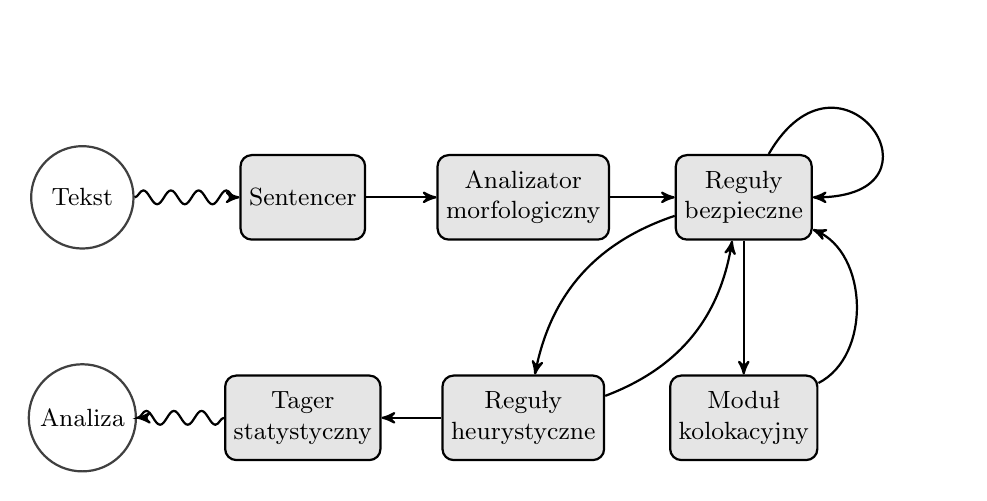
\begin{tikzpicture}[node distance=2.8cm, auto]\small
\tikzset{every loop/.style={min distance=10mm,in=0,out=60,looseness=6}}
\tikzstyle{block} = [rectangle, draw, thick, fill=gray!20,
  text centered, rounded corners, minimum height=3.3em, minimum width=4em]
\tikzstyle{line} = [-stealth', thick, draw]
\tikzstyle{tekst} = [circle,thick,draw=black!75,fill=white,minimum size=1.3cm]

    \node [tekst] (tekst) {Tekst};
    \node[align=center] [block,right of=tekst] (sentencer) {Sentencer};
    \node[align=center] [block,right of=sentencer] (analizator) {Analizator\\morfologiczny};
    \node[align=center] [block,right of=analizator] (reg-pewne) {Reguły\\bezpieczne};
    \node[align=center] [block,below of=reg-pewne] (phras) {Moduł\\kolokacyjny};
    \node[align=center] [block,left of=phras] (reg-heur)
    {Reguły\\heurystyczne};
    \node[align=center] [block,left of=reg-heur] (tager) {Tager\\
      statystyczny};
    \node [tekst,left of=tager] (analiza) {Analiza};
    \path [line,decorate, decoration=snake] (tekst) -- (sentencer);
    \path [line] (sentencer) -- (analizator);
    \path [line] (analizator) -- (reg-pewne);
    \path [line] (reg-pewne) edge [loop above] ();
    \path [line] (reg-heur) edge [bend right=30] (reg-pewne);
    \path [line] (reg-pewne) edge [bend right=30] (reg-heur);
    \path [line] (reg-pewne) -- (phras);
    \path [line] (phras) edge [bend right=65] (reg-pewne);
    \path [line] (reg-heur) -- (tager);
    \path [line,decorate, decoration=snake] (tager) -- (analiza);
\end{tikzpicture}
\framebreak

Komponenty:
\begin{itemize}
\item obszerny słownik (ok. 800 000 haseł, w~tym ok. 200 000 nazw własnych),
\item duży zestaw reguł (ok. 2600) tworzonych ręcznie w~formalizmie \emph{LanGr},
\item moduł kolokacyjny \emph{Phras},
\item analizatory statystyczne \emph{MorČe} i~\emph{MorphoDiTa}.
\end{itemize}

\end{frame}

\begin{frame}
  \frametitle{Możliwe zastępniki}

Polskie zasoby, które (potencjalnie) można wykorzystać:
\begin{itemize}
\item \href{http://sgjp.pl/}{SGJP} (ew. Polimorf), być może rozszerzony o~więcej nazw
  własnych, np. wszystkie nazwiska z~bazy PESEL,
\item Spejd,
\item \emph{Słownik elektroniczny jednostek frazeologicznych} (\href{http://zil.ipipan.waw.pl/SEJF}{SEJF}),
\item \emph{Słownik paradygmatów polskich frazeologizmów czasownikowych} (\href{http://uwm.edu.pl/verbel/}{VERBEL}),
\item być może również ramki frazeologiczne Walentego (?),
\item omówione wcześniej tagery statystyczne.
\end{itemize}


\end{frame}

\begin{frame}%[allowframebreaks]
  \frametitle{SEJF}

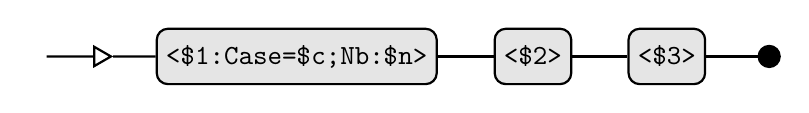
\begin{tikzpicture}[node distance=3.8cm,auto]
  \tikzstyle{block} = [rectangle, draw, thick, fill=gray!20,
  text centered, rounded corners, minimum height=2em, minimum width=2.5em]
  \tikzstyle{dot} = [circle,draw,fill=black,inner sep=0pt,minimum size=8pt]
  \tikzstyle{triangle} = [regular polygon,regular polygon sides=3,draw,fill=white,rotate=30,thick,inner sep=0pt,minimum size=8pt]
  \tikzstyle{line} = [thick, draw]
\node (0) at (-1.3,1) {};
\node [triangle] (tri) at (-.5,1) {};
\node [block] (1) at (2,1) {\texttt{<\$1:Case=\$c;Nb:\$n>}};
\node [block] (2) at (5,1) {\texttt{<\$2>}};
\node [block] (3) at (6.7,1) {\texttt{<\$3>}};
\node [dot] (4) at (8,1) {};
\path [line] (0) -- (tri);
\path [line] (tri) -- (1);
\path [line] (1) -- (2);
\path [line] (2) -- (3);
\path [line] (3) -- (4);
%\draw (t1) -- (t2) -- (t3) -- (t4);
\end{tikzpicture}

\[\scriptsize
\underbrace{\text{akt
    \texttt{[akt:subst:sg:nom:m3]}}}_{\text{\$1}}\underbrace{\phantom{Fg}}_{\text{\$2}}
\underbrace{\text{oskarżenia \texttt{[oskarżenie:subst:sg:gen:n2]}}}_{\text{\$3}}
\]

Przykładowe zastosowanie:
\begin{itemize}
%Pantera:\\
\item (...) skierowano do sądu \textbf{akt} \texttt{\small[akta:subst:pl:gen:n]} oskarżenia.

%WMBT
\item (...)
%listu gończego dołącza się
odpisy aktu \textbf{oskarżenia} \texttt{\small [ger:sg:gen:n:perf:aff]} (...)
\end{itemize}
\end{frame}


\begin{frame}
\frametitle{SEJF}
W~NKJP300 jest 4116 ciągów pasujących do zapytania
\texttt{[base\textapprox "akt"] [base\textapprox "oskarżenie"]}. Ale tylko 2182 spełnia
warunki nałożone na to wyrażenie w~SEJF-ie. Reszta to błędy, zwykle
polegające na wyborze rzeczownika \textsc{akta}.

\bigskip
\pause

Podobnie dla \texttt{[base\textapprox"armia"] [base\textapprox"czerwony"]} --- 1983
wyników, ale tylko 120 spełnia ograniczenia SEJF-u. Reszta to
w~większości błędy polegające na wyborze rzeczownika
\textsc{czerwona}.

\bigskip
\pause

Dla ciągu \texttt{[base\textapprox"brud"] [base=","]
  [base\textapprox"smród"] [base="i"] [base\textapprox"ubóstwo"]}
Pantera uparcie wybiera rzeczownik \textsc{smród} \textsc{m1}. Jedyne
poprawne dopasowanie jest w~dopełniaczu.

\end{frame}


\section{Dyskusja i rekomendacje}
\frame{\sectionpage}

\begin{frame}
  \frametitle{Możliwe ulepszenia}

  \begin{itemize}
  \item Uspójnienie korpusu treningowego ze słownikiem.
  \item Zwiększenie ilości danych treningowych.
  \item Rozszerzanie słownika o~nazwy własne.
  \item Wykorzystanie dodatkowej informacji słownikowej
    (kwalifikatory, pospolitość).
  \item Wykorzystanie innych zasobów lingwistycznych obejmujących
    np. frazeologię.
  \item Zastosowanie ręcznie pisanych reguł \pauza przynajmniej do
    kontroli jakości znakowania.
  \end{itemize}


\end{frame}


\begin{frame}{Struktura danych treningowych w NKJP1M}

% Tutaj powiem dwa słowa o~tym, że inne tagery są trenowane na
% bardziej jednolitych tekstach i~że można spróbować eksperymentów
% z~trenowaniem bez internetów i~podkorpusu mówionego.

  \begin{center}
    \includegraphics[scale=0.7]{img/nkjp1m.png}
  \end{center}


\end{frame}

\begin{frame}{Podsumowanie}
  \structure{Cechy pożądanego tagera (M. Woliński)}
  \vspace{0.5cm}

  Chciałbym tager, który:
   \begin{itemize}
   \item<1-> nie jest nadgorliwy, można kazać zostawić interpretacje częściowo nieujednoznacznione (np. usunąć tylko bardzo złe interpretacje),\\
   \alert{obecnie: Pantera, Concraft; po zmianie parametru: WCRFT, WMBT,}
   \item<2-> informuje o~poziomie pewności podjętych decyzji,\\
   \alert{obecnie: Concraft, możliwe: WCRFT, WMBT; trudniejsze dla Pantery}
   \item<3-> działa na niejednoznacznej segmentacji (stworzonej przez Morfeusza lub np. będącej wynikiem zastosowania po Morfeuszu słownika wyrażeń wieloczłonowych),\\
   \alert{obecnie: tylko tagset pośredni, możliwe: w każdym po modyfikacjach całego stosu,}
   \end{itemize}
\end{frame}

\begin{frame}{Podsumowanie (2)}
  \structure{Cechy pożądanego tagera (M. Woliński)}
  \vspace{0.5cm}

  Chciałbym tager, który:
   \begin{itemize}
    \item<1-> daje się (względnie?) łatwo zainstalować i uruchomić na wszystkich platformach, na których jest Morfeusz,\\
    \alert{obecnie: żaden; trzeba przygotować dystrybucję binarną Macy pod Windows; Haskell Platform + Concraft lub kompilacja innych tagerów,}
    \item<2-> da się rozszerzyć o uwzględnianie informacji o czasie powstania tekstu,\\
    \alert{obecnie: żaden, możliwe: w opartych na ML jako dodatkowa cecha.}
  \end{itemize}
\end{frame}

\begin{frame}{Podziękowania}
  \structure{Podziękowania za sugestie i uwagi dla:}
  \begin{itemize}
    \item Adama Radziszewskiego
    \item Jakuba Waszczuka
    \item Szymona Acedańskiego
  \end{itemize}
\end{frame}

\begin{frame}{}
\begin{centering}
    \begin{beamercolorbox}[sep=12pt,center]{part title}
    \usebeamerfont{section title}Dziękujemy za uwagę!\par
    \end{beamercolorbox}
    \end{centering}
\end{frame}

\begin{frame}{Tagowanie języka angielskiego}
  \structure{Penn Treebank Wall Street Journal (WSJ) release 3}
  \footnotesize
  \begin{tabular}{cp{3.5cm}p{2.5cm}c}
    System & Metoda & Publikacja & Dokładność \\ \hline
    BI-LSTM-CRF & Bidirectional LSTM-CRF Model & Huang et al. (2015) & 97.55 \\ \hline
    SCCN & Semi-supervised condensed nearest neighbor & Søgaard (2011) & 97.50 \\ \hline
    Morče/COMPOST & Averaged Perceptron & Spoustová et al. (2009) & 97.44 \\ \hline
    structReg & CRFs with structure regularization & Sun(2014) & 97.36 \\ \hline
    LTAG-spinal & Bidirectional perceptron learning & Shen et al. (2007) & 97.33 \\ \hline
    Stanford Tagger 2.0 & Maximum entropy cyclic dependency network & Manning (2011) & 97.32 \\ \hline
    Stanford Tagger 2.0 & Maximum entropy cyclic dependency network & Manning (2011) & 97.29 \\ \hline
    Stanford Tagger 1.0 & Maximum entropy cyclic dependency network & Toutanova et al. (2003) & 97.24 \\ \hline
  \end{tabular}
\end{frame}

\begin{frame}{Tagowanie języka angielskiego}
  \footnotesize
  \begin{tabular}{cp{3.5cm}p{2.5cm}c}
    System & Metoda & Publikacja & Dokładność \\ \hline
    Morče/COMPOST & Averaged Perceptron & Spoustová et al. (2009) & 97.23 \\ \hline
    LAPOS & Perceptron based training with lookahead & Tsuruoka, Miyao, and Kazama (2011) & 97.22 \\ \hline
    SVMTool & SVM-based tagger and tagger generator & Giménez and Márquez (2004) & 97.16 \\ \hline
    Maxent easiest-first & Maximum entropy bidirectional easiest-first inference & Tsuruoka and Tsujii (2005) & 97.15 \\ \hline
    Averaged Perceptron & Averaged Perception discriminative sequence model & Collins (2002) & 97.11 \\ \hline
    GENiA Tagger** & Maximum entropy cyclic dependency network & Tsuruoka, et al (2005) & 97.05 \\ \hline
    MElt & MEMM with external lexical information & Denis and Sagot (2009) & 96.96 \\ \hline
    TnT* & Hidden markov model & Brants (2000) & 96.46 \\ \hline
\end{tabular}
\end{frame}

\begin{frame}[allowframebreaks]
  \frametitle{Bibliografia}
  \begin{thebibliography}{10}
  \beamertemplatebookbibitems
  \bibitem[Acedański, 2010]{ace:2010}
Acedański, Szymon, 2010.
\newblock A morphosyntactic {B}rill tagger for inflectional languages.
\newblock In {\em Advances in Natural Language Processing\/}.
  \beamertemplatearticlebibitems
  \bibitem[Brill and Wu, 1998]{bri:wu:1998}
Brill, Eric and Jun Wu, 1998.
\newblock Classifier combination for improved lexical disambiguation.
\newblock In {\em Proceedings of the 17th international conference on
  Computational linguistics - Volume 1\/}, COLING '98. Stroudsburg, PA, USA:
  Association for Computational Linguistics.
  \beamertemplatearticlebibitems
  \bibitem[Śniatowski and Piasecki, 2012]{sni:pia:2012}
Śniatowski, Tomasz and Maciej Piasecki, 2012.
\newblock Combining {P}olish morphosyntactic taggers.
\newblock In Pascal Bouvry, Mieczysław~A. Kłopotek, Franck Leprévost,
  Małgorzata Marciniak, Agnieszka Mykowiecka, and Henryk Rybiński (eds.),
  {\em Security and Intelligent Information Systems\/}, volume 7053 of {\em
  LNCS\/}. Springer-Verlag.
  \beamertemplatearticlebibitems
  \bibitem[Radziszewski, 2013]{rad:2013}
Radziszewski, Adam, 2013.
\newblock A tiered {CRF} tagger for {P}olish.
\newblock In R.~Bembenik, {\L}.~Skonieczny, H.~Rybi\'{n}ski, M.~Kryszkiewicz,
  and M.~Niezg{\'o}dka (eds.), {\em Intelligent Tools for Building a Scientific
  Information Platform: Advanced Architectures and Solutions\/}. Springer
  Verlag.
  \beamertemplatearticlebibitems
  \bibitem[Radziszewski and Acedański, 2012]{rad:ace:2012}
Radziszewski, Adam and Szymon Acedański, 2012.
\newblock {T}aggers gonna tag: an argument against evaluating disambiguation
  capacities of morphosyntactic taggers.
\newblock In {\em Proceedings of TSD 2012\/}, LNCS. Springer-Verlag.
\beamertemplatearticlebibitems
\bibitem[Radziszewski and Śniatowski, 2011a]{rad:sni:2011}
Radziszewski, Adam and Tomasz Śniatowski, 2011a.
\newblock {A} {M}emory-{B}ased {T}agger for {P}olish.
\newblock In {\em Proceedings of the LTC 2011\/}.
\beamertemplatearticlebibitems
\bibitem[van Halteren et~al., 2001]{hal:dae:zav:2001}
van Halteren, Hans, Walter Daelemans, and Jakub Zavrel, 2001.
\newblock Improving accuracy in word class tagging through the combination of
  machine learning systems.
\newblock {\em Comput. Linguist.\/}, 27(2):199--229.
\beamertemplatearticlebibitems
\bibitem[Waszczuk, 2012]{wasz:12}
Waszczuk, Jakub, 2012.
\newblock Harnessing the {CRF} complexity with domain-specific constraints.
  {T}he case of morphosyntactic tagging of a highly inflected language.
\newblock In {\em Proceedings of the 24th International Conference on
  Computational Linguistics ({COLING}\,2012)\/}. Mumbai, India.
  \end{thebibliography}
\end{frame}

\end{document}
